% !TEX root = ../main.tex
\paragraph{Tracking}
% --+ Introduction +------------------------------------------------------------
    \begin{wrapfigure}{r}{0.50\textwidth}
        \centering\frame{
        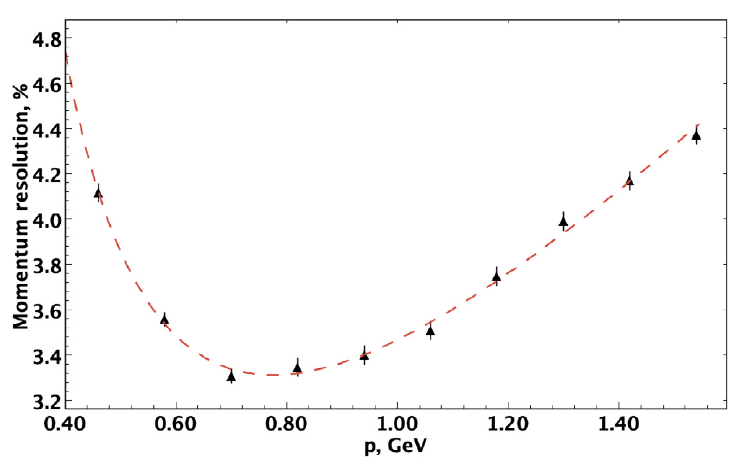
\includegraphics[width=\linewidth]{11experiment/img/231cvt_pres.png}}
        \caption[CVT momentum resolution vs. momentum.]{Momentum resolution vs. momentum of simulated protons in the CVT without background.}
        \label{fig::cvt_pres}
    \end{wrapfigure}

    In the CLAS12 event reconstruction, charged particle tracking plays a crucial role and is divided into two main regions: the forward region and the central region.

    In the forward region, charged particles are bent either inward or outward from the beamline by the torus magnet, depending on their charge.
    The magnetic field strength varies along the bending path, with an integral magnetic field ($\int Bdl$) ranging from $2 \text{Tm}$ at $5\degree$ to $0.5 \text{Tm}$ at $40\degree$.
    The forward tracking system responsible for tracking in this region consists of two components: the Forward MicroMegas Tracker (FMT) and the Drift Chambers (DC).

    In the central region, charged tracks are curved into helices by the strong $5 \text{T}$ solenoidal magnetic field.
    The central tracking system comprises the Silicon Vertex Tracker (SVT) and the Barrel MicroMegas Tracker (BMT), which together form the Central Vertex Tracker (CVT).

    These tracking systems in both the forward and central regions use sophisticated detectors to measure the position of charged particle hits, allowing for the reconstruction of particle trajectories.
    By combining information from these detectors and utilizing the magnetic field information, the tracking algorithms reconstruct the paths of charged particles, enabling precise determination of their momenta and vertices.

% --+ Reconstruction +----------------------------------------------------------
    In both the forward and central tracking systems, track reconstruction involves two main steps: pattern recognition and track fitting.
    The first step is to identify hits, which are the recorded signals corresponding to a particle passing through a specific detector component.
    These hits are transformed from electronic signals into the position of the track within the geometry of the detector subsystem.

    \begin{wrapfigure}{r}{0.50\textwidth}
        \centering\frame{
        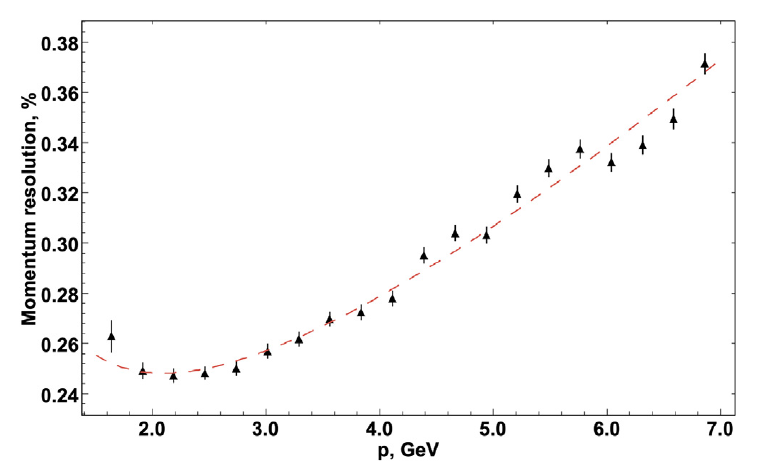
\includegraphics[width=\linewidth]{11experiment/img/231dc_pres.png}}
        \caption[DC momentum resolution vs momentum.]{Momentum resolution vs. momentum in the DC evaluated using pions simulated at $\theta = 15\degree \pm 5\degree$ and at $\phi = 0 \pm 5\degree$ without background.}
        \label{fig::dc_pres}
    \end{wrapfigure}


    A hit is defined as a geometric object that represents a detector element.
    For example, in the central tracker, a hit can be represented by a line corresponding to a strip in the detector.
    These hit objects serve as the input for the pattern recognition algorithms.

    \begin{figure}[t]
        \centering\frame{
        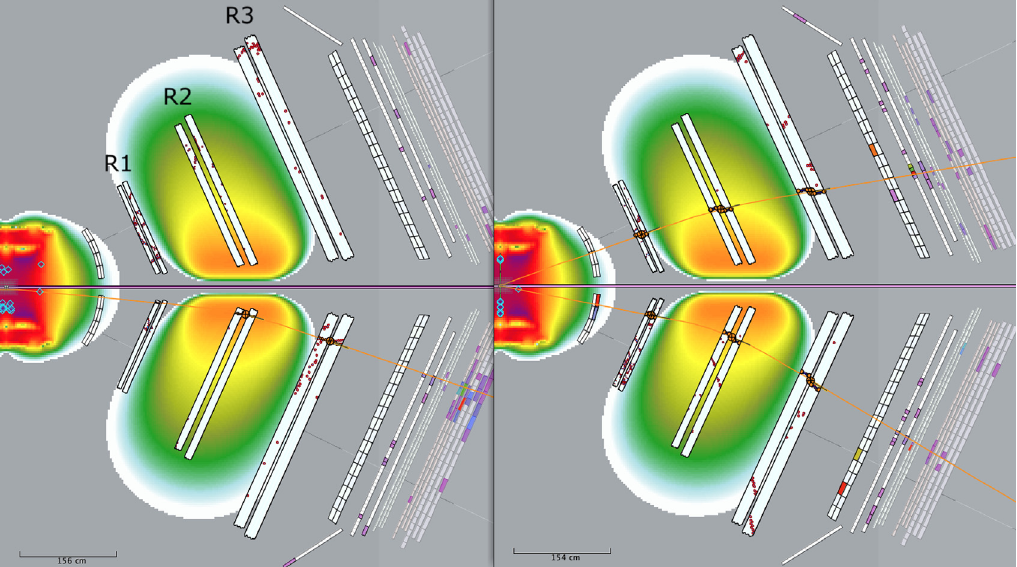
\includegraphics[width=\textwidth]{11experiment/img/231ced_event.png}}
        \caption[Particle going through DC.]{Views from CLAS12 Event Display (ced) of charged particle tracks in the DC showing cut-views to highlight different pairs of sectors of the CLAS12 Forward Detector.
        The coloured detector elements are the registered hits and the orange lines are the result of track reconstruction using the hits in the DC.
        The coloured areas about the detectors represent the regions of magnetic field from the torus and the solenoid.
        In these views the beam is incident from the left and the target is located in the middle of the solenoid (at the left edge of the image).}
        \label{fig::ced_event}
    \end{figure}
    Pattern recognition involves identifying clusters of hits and determining the spatial coordinates and corresponding uncertainties for the hits and clusters.
    During the pattern recognition stage, hits that are consistent with belonging to a trajectory, such as a particle track, are identified.
    This set of hits is then fitted to the expected trajectory, considering their uncertainties and incorporating knowledge of the detector material and the detailed magnetic field map.
    Figure \ref{fig::ced_event} illustrates a particle passing through the DC.

% --+ Performance +-------------------------------------------------------------
    The momentum resolutions in the central and forward trackers, as a function of momentum, are shown in Figures \ref{fig::cvt_pres} and \ref{fig::dc_pres}, respectively.
    The distributions are fitted with a function of the form $\sqrt{a + bx^2 + c/(1 + d/x^2)}$.
    In both distributions, the degradation of resolution at low momentum is attributed to multiple scattering effects.
    Furthermore, the resolution deteriorates as momentum increases beyond a minimum, primarily because of poorer track curvature resolution.

    For central tracking, a simulated proton sample with momenta ranging from $0.5$ to $2.5 \text{ GeV}$ yields an average CVT reconstruction efficiency of $87.3\%$.
    A slight decrease in efficiency is observed for tracks with momenta below $600 \text{ MeV}$.
    The increased curvature of low transverse momentum ($\text{p}_\perp$) tracks leads to a rise in inefficiency due to acceptance effects.
    The primary source of inefficiency stems from the gaps between the sensitive volumes of the BMT and SVT detectors.

    Regarding forward tracking, the momentum resolution in the DC is evaluated using tracks simulated at $\theta = 15\degree \pm 5\degree$ and $\phi = 0 \pm 5\degree$.
    This range ensures that the majority of tracks fall within the sensitive volume.
    Moreover, the DC momentum resolution exhibits correlation with the polar angle since track curvature is determined by the magnetic field intensity, which is higher at lower angles in the torus field.
    These resolutions are obtained from a Monte Carlo sample that excludes out-of-time backgrounds or misalignments of the tracking volumes \cite{ziegler2020}.
